% tcm-less.tex

\documentclass{standalone}

\usepackage{tikz}
\usetikzlibrary{shapes, positioning, arrows.meta, decorations.pathmorphing}

\begin{document}
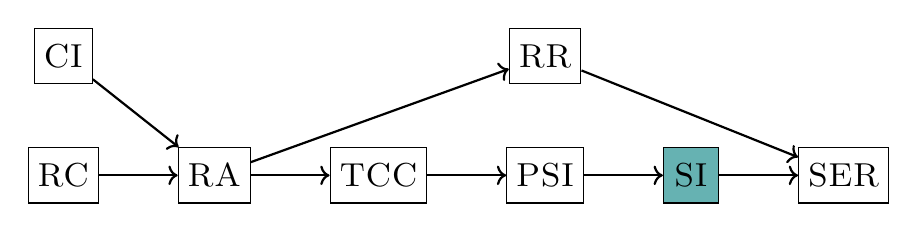
\begin{tikzpicture}[model/.style = {draw, minimum size = 20pt, font = \large},
  edge/.style = {->, thick},
  node distance = 0.8cm and 1.0cm]

  \node[model] (rc) {\textsc{RC}};
    \node[model, above = of rc] (ci) {\textsc{CI}};
  \node[model, right = of rc] (ra) {\textsc{RA}};
  \node[model, right = of ra] (tcc) {\textsc{TCC}};
  \node[model, right = of tcc] (psi) {\textsc{PSI}};
  \node[model, right = of psi, fill = teal!60] (si) {\textsc{SI}};
    \node[model, above = of psi] (rr) {\textsc{RR}};
  \node[model, right = of si] (ser) {\textsc{SER}};

  \draw[every edge, ->, thick]
    (ci) edge (ra)
    (rc) edge (ra)
    (ra) edge (tcc)
       edge (rr)
       (rr) edge (ser)
    (tcc) edge (psi)
    (psi) edge (si)
    (si) edge (ser);
\end{tikzpicture}
\end{document}